\documentclass{standalone}
\usepackage{tikz}
\usepackage{verbatim}
\usetikzlibrary{positioning}
\begin{document}
\pagestyle{empty}
  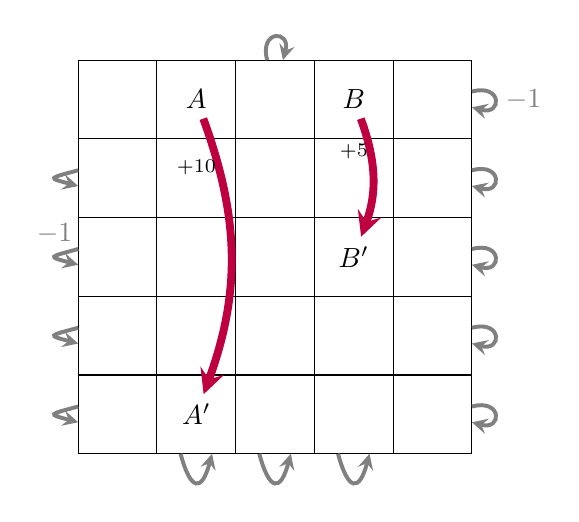
\begin{tikzpicture}
    \draw[step=1.0,black,thin] (0,0) grid (5, 5);
    \node (a) at (1.5, 4.5) {$A$};
    \node (ap) at (1.5, 0.5) {$A'$};
    \path[-stealth,purple,line width=1mm] (a) edge[bend left = 20] (ap);
    \node (b) at (3.5,4.5) {$B$};
    \node (bp) at (3.5, 2.5) {$B'$};
    \path[-stealth,purple,line width=1mm] (b) edge[bend left = 20] (bp);
    \node[below = 2mm of b] {$\scriptstyle +5$};
    \node[below = 4mm of a] {$\scriptstyle +10$};
    \foreach \x in {1.5, 2.5, 3.5} {
      \path[-stealth,line width=0.5mm] (\x-0.2, 0) edge[loop below,gray,distance=5mm] (\x+0.2, 0);
    }
    \path[-stealth,line width=0.5mm] (5, 4.6) edge[loop right,gray,distance=4mm] node[right] {$-1$}       (5, 4.4);
    \foreach \y in {3.5, 2.5, 1.5, 0.5} {
      \path[-stealth,line width=0.5mm] (5, \y+.1) edge[loop right,gray,distance=4mm] (5, \y-.1);
      \path[-stealth,line width=0.5mm] (0, \y+.1) edge[loop left ,gray,distance=4mm] (0, \y-.1);
    }
    \path[-stealth,line width=0.5mm] (2.4, 5) edge[loop above,gray,distance=4mm] (2.6, 5);
    \node[gray] at (-0.3, 2.8) {$-1$};
  \end{tikzpicture}
\end{document}